
% \subsection{INSTITUTIONAL SHIFTS AND STRUCTURES}
\subsection{分水制度与流域SES构件的演变}\label{results-1}

\begin{figure}[!t]
	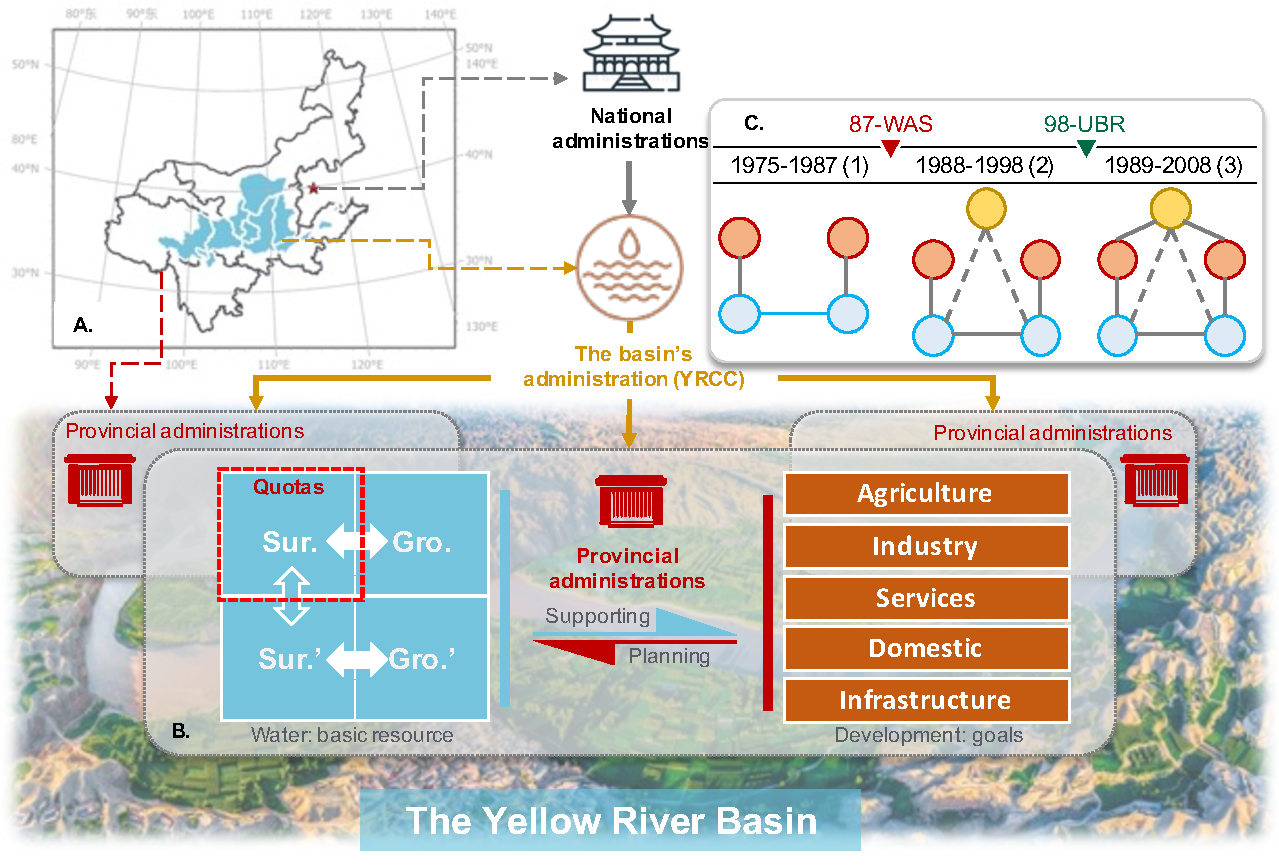
\includegraphics[width=\linewidth]{img/ch5/diagram.pdf}
	\caption[黄河流域社会经济制度变迁及其结构]{
		黄河流域社会经济制度变迁及其结构。
		\textbf{A.} 黄河流域跨越$10$个省(地区),其中$8$个对黄河流域水资源的依赖程度较高。国家部委(水利部)是发布水治理政策的最高权力机构,这些政策通常由流域级机构黄河水利委员会和各省级机构执行。
		\textbf{B.} 地方省政府(水利厅、局)是水分方案中的主要的利益相关者。自“八七”分水方案以来,由于黄河地表水的取用受到配额限制,利益相关者规划和利用水资源进行发展受到影响。自然水文过程是相互联系的,尽管配额制度主要限制地表水($Sur$),也可能通过社会水文过程影响流域内地下水($Gro$)或流域外水资源($Sur'$和$Gro'$)。
		\textbf{C.} 制度变迁和随之而来的社会-生态系统结构变化:
		(1) $1979 \sim 1987$年间,各利益相关方(红圈)从连接的生态单元(黄河河段,蓝圈)自由获取水资源。
		(2) 1987年施行“八七”分水方案后,黄河水利委员会(黄圈)负责监测各河段利益相关者用水情况。
		(3) 1998年施行“流域统一调度”之后,利益相关者必须向黄河水利委员会申请用水许可证(红黄圈之间的连接)。}\label{fig:structure}
\end{figure}

% 制度变动综述
1987年实施的“八七”分水方案和1998年实施的“流域统一调度”是黄河流域水治理中被广泛认可的里程碑事件。
在“八七”分水方案之前,分水方案的利益相关者(参与分水的黄河流域各省份或地区)可以根据其取水能力自由使用黄河的水资源进行开发,流域管理机构(黄河水利委员会)与利益相关者在用水方面没有联系(图~\ref{fig:structure}~C)。
为缓解水资源压力,国家部委在“八七”分水方案中提出黄河流域$10$个省(或地区)之间应参照指定配额来取用水资源,且该配额与各省的预期取水量相去甚远(表~\ref{ch5:tab:quota})。
同时根据官方文件中的要求,流域尺度机构黄河水利委员会需开始报告各省(或地区)和各个河段的用水情况,这是黄河流域水利枢纽的责任首次涉及水资源利用,在社会与生态节点之间引入了新的联系(图~\ref{fig:structure}~C)。
由于备受争议的“八七”分水方案在此后十年内都没能解决黄河断流问题,1998年水利部签署同意了另一项制度改革——流域统一调度,强化了黄河水利委员会在综合管理用水方面的职责。
此次官方文件明确指出,各省须将其年度用水计划向黄河水利委员会报备并申请用水许可证,否则不再能使用黄河干流水资源,黄河水利委员会因此在社会-生态系统结构中同各省直接联系在一起(图~\ref{fig:structure}~C)。
综上所述,两次制度转换重塑了黄河流域水资源利用的结构,形成的三类具一般性的社会-生态系统结构块如图~\ref{fig:structure}~C所示。

% Table generated by Excel2LaTeX from sheet '八七分水方案配额'
\begin{table}[htbp]
    \caption{八七分水方案水资源配额}
      \begin{tabularx}{\textwidth}{p{2cm} LLLLLLLLLL}
      \toprule
            & \multicolumn{1}{l}{青海} & \multicolumn{1}{l}{四川$^b$} & \multicolumn{1}{l}{甘肃} & \multicolumn{1}{l}{宁夏} & \multicolumn{1}{l}{内蒙古} & \multicolumn{1}{l}{山西} & \multicolumn{1}{l}{陕西} & \multicolumn{1}{l}{河南} & \multicolumn{1}{l}{山东} & \multicolumn{1}{l}{津冀$^b$} \\
      \midrule
      规划需求  & 35.7  & 0     & 73.5  & 60.5  & 148.9 & 115   & 60.8  & 111.8 & 84    & 6 \\
      1983年方案 & 14    & 0     & 30    & 40    & 62    & 43    & 52    & 58    & 75    & 0 \\
      1987年方案 & 14.1  & 0.4   & 30.4  & 40    & 58.6  & 38    & 43.1  & 55.4  & 70    & 20 \\
      多年平均耗水$^a$ & 12.03 & 0.25  & 25.8  & 36.58 & 61.97 & 21.16 & 11.97 & 34.3  & 77.87 & 5.85 \\
      黄河水在地区总用水的占比 & 48.12\% & 0.10\% & 30.79\% & 58.45\% & 47.82\% & 73.55\% & 44.39\% & 24.77\% & 34.41\% & 3.11\% \\
      \bottomrule
      \end{tabularx}\label{ch5:tab:quota}%
      \footnotesize
      \\
      $a$ 使用1987年到2008年数据计算,四川因数据不足,使用2004到2017年数据计算。\\
      $b$ 由于取自黄河流域的水资源占省(或地区)总用水量的比值太小($< 5\%$),不在本研究中进行考虑。
\end{table}%


\subsection{主成分提取结果}

具有解释力的变量是构建稳健的合成控制方法的关键。
我们使用了与用水相关的24个变量(见表~\ref{ch5:tab:data_source}),这些数据集在先前的研究中已用于解释中国用水的变化\cite{zhou2020}。
由于这些变量之间存在自相关性,我们使用肘部法选择了5个主成分作为DSC的输入,以减少维数并增强合成控制方法的稳健性(见图~\ref{ch5:fig:elbow})。

\begin{figure}[htb]
    \centering
    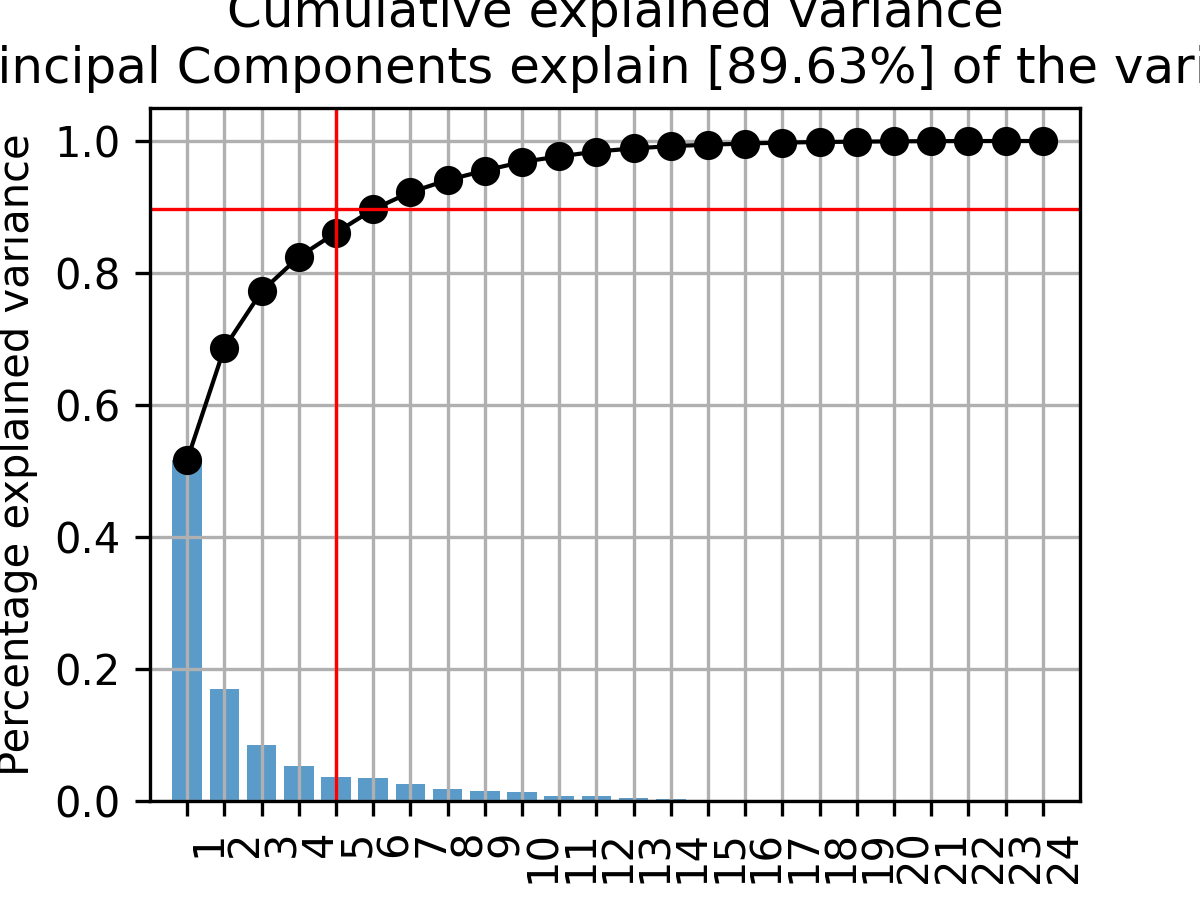
\includegraphics[width=0.6\textwidth]{img/ch5/ch5_elbow.png}
    \caption{主成分分析肘部图}\label{ch5:fig:elbow}
\end{figure}

\subsection{合成控制结果}

对DSC的有效性测试有两种方法:(1)比较后期和前期的重建;(2)通过安慰剂分析测试鲁棒性。
对于(1),每个省份和它们的合成后期差异显著,而在合成前期差异较小(见图~\ref{fig:87panel}和图~\ref{fig:98panel}),这表明其水消耗变化的估计重建良好。
对于(2),我们采用了\cite{abadie2010}所描述的现场安慰剂分析。在大多数省份中,合成后期 MSPE 与合成前期 MSPE 的比率高于其他安慰剂单位的中位数,这表明在治疗时间(此处为1987年和1998年)发生的制度转变比大多数其他省份影响更大(见图~\ref{fig:87placebo},图~\ref{fig:98placebo}和表~\ref{tab:DSC_summary})。


\begin{table*}
	\caption{Pre and post treatment root mean squared prediction error (RMSPE) for YRB's provinces}
	\label{tab:DSC_summary}
	\scriptsize
	\centering
	\resizebox{\linewidth}{!}{
	\begin{tabular}{lrrrrrrrr}
	\hline
	 & \multicolumn{4}{c}{1987-WAS} & \multicolumn{4}{c}{1998-UBR} \\
	 Provinces & Pre-RMSPE & Post-RMSPE & Ratio & Significant$^a$ & Pre-RMSPE & Post-RMSPE & Ratio & Significant$^a$ \\
	 \hline
	 Qinghai & 0.016 & 0.231 & 14.606 & True & 0.230 & 1.170 & 5.096 & True \\
	Gansu & 0.056 & 1.307 & 23.265 & True & 0.244 & 0.841 & 3.448 & True \\
	Ningxia & 0.097 & 0.944 & 9.697 & True & 0.332 & 1.091 & 3.284 & True \\
	Neimeng & 0.335 & 3.846 & 11.479 & True & 1.320 & 1.183 & 0.896 & False \\
	Shanxi & 0.208 & 0.675 & 3.241 & False & 0.264 & 0.401 & 1.520 & False \\
	Shaanxi & 0.181 & 0.572 & 3.164 & False & 0.096 & 0.724 & 7.579 & True \\
	Henan & 0.210 & 3.207 & 15.292 & True & 1.222 & 2.479 & 2.029 & False \\
	Shandong & 0.209 & 1.840 & 8.785 & True & 0.431 & 1.517 & 3.516 & True \\
	\hline
	\end{tabular}}
	\footnotesize[a]\leftline{{Larger post/pre RMSPE than the median of the placebos.}}\\
\end{table*}



\begin{figure}[!bh]
    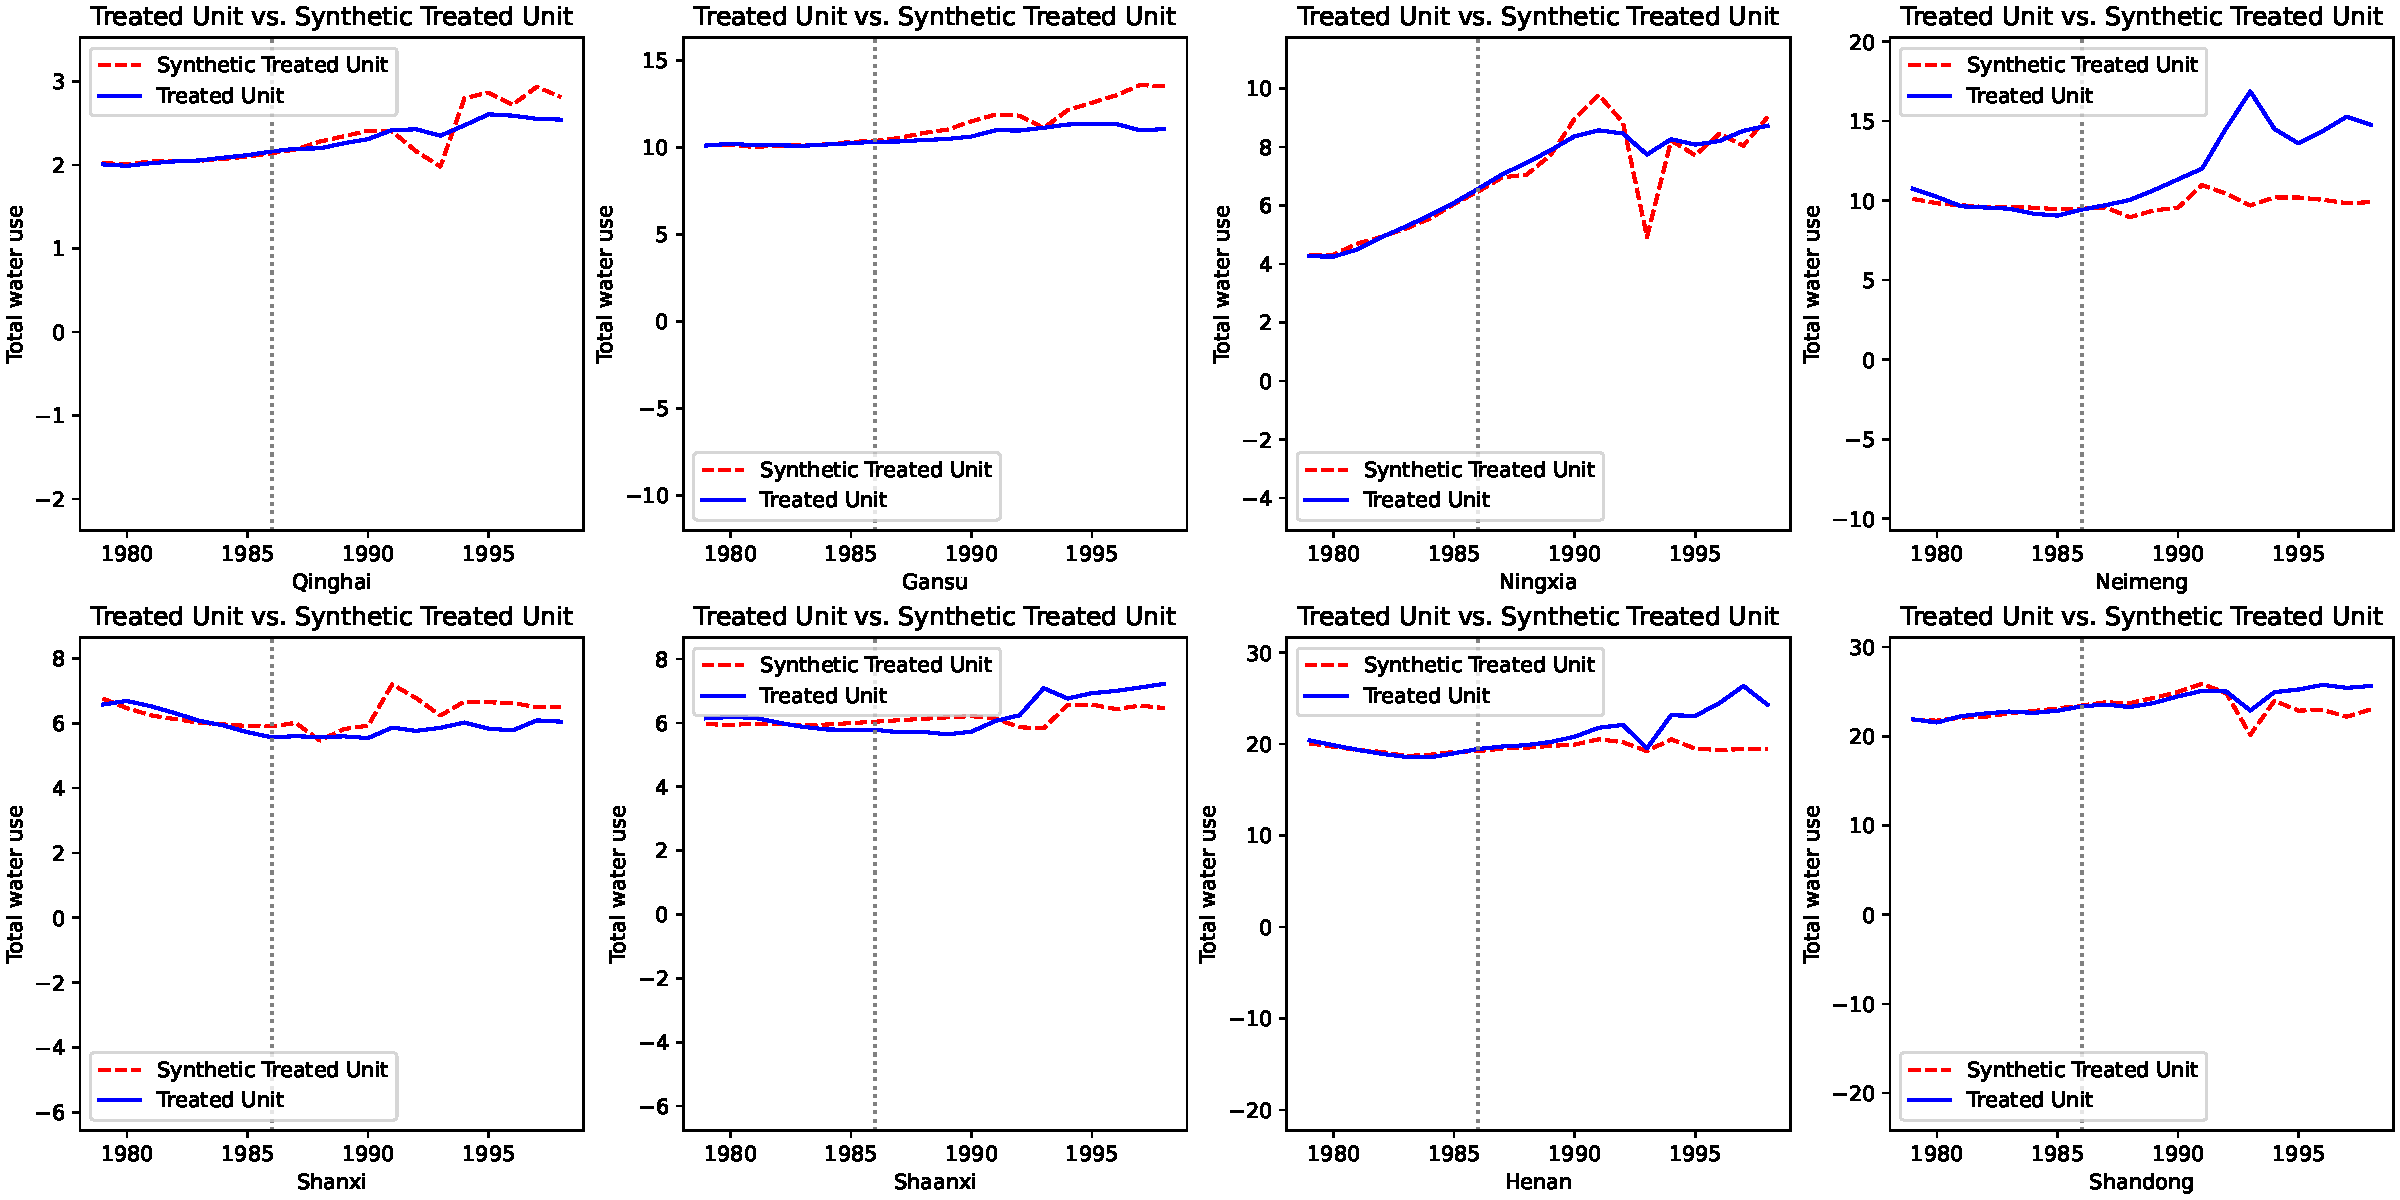
\includegraphics[width=0.9\linewidth]{img/ch5/87panel.pdf}
    \centering
    \caption[“八七”分水制度前后的合成控制对照]{“八七”分水制度前后黄河流域各省份和它们合成控制对照的用水量对比}\label{fig:87panel}
\end{figure}

\begin{figure}
    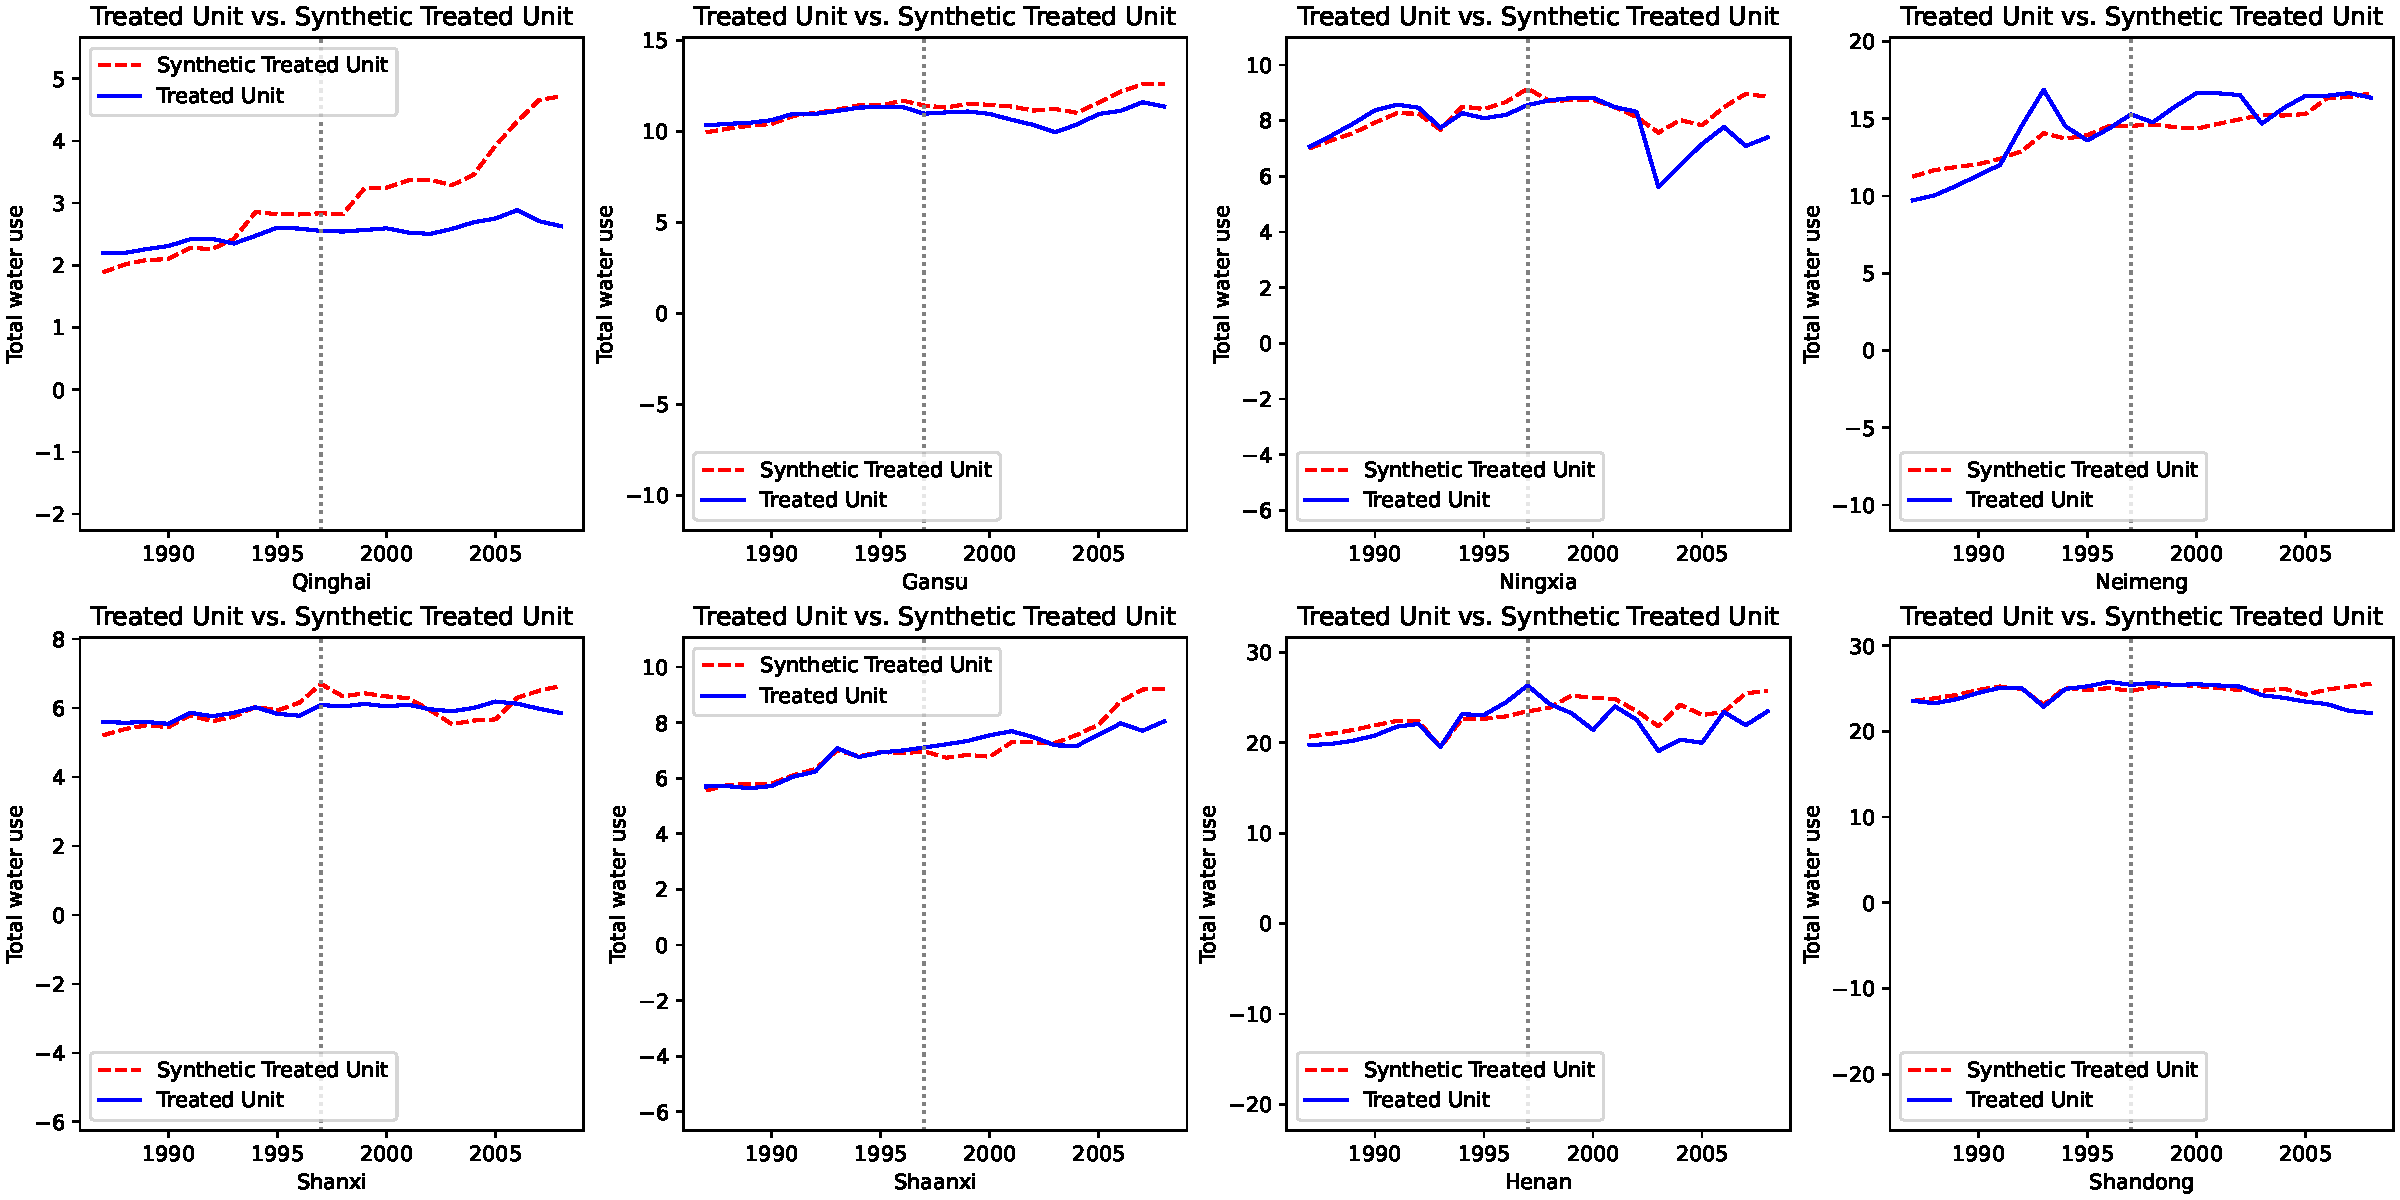
\includegraphics[width=0.9\linewidth]{img/ch5/98panel.pdf}
    \centering
    \caption[流域统一调度制度前后的合成控制对照]{流域统一调度制度前后黄河流域各省份和它们合成控制对照的用水量对比}\label{fig:98panel}
\end{figure}


\begin{figure}
    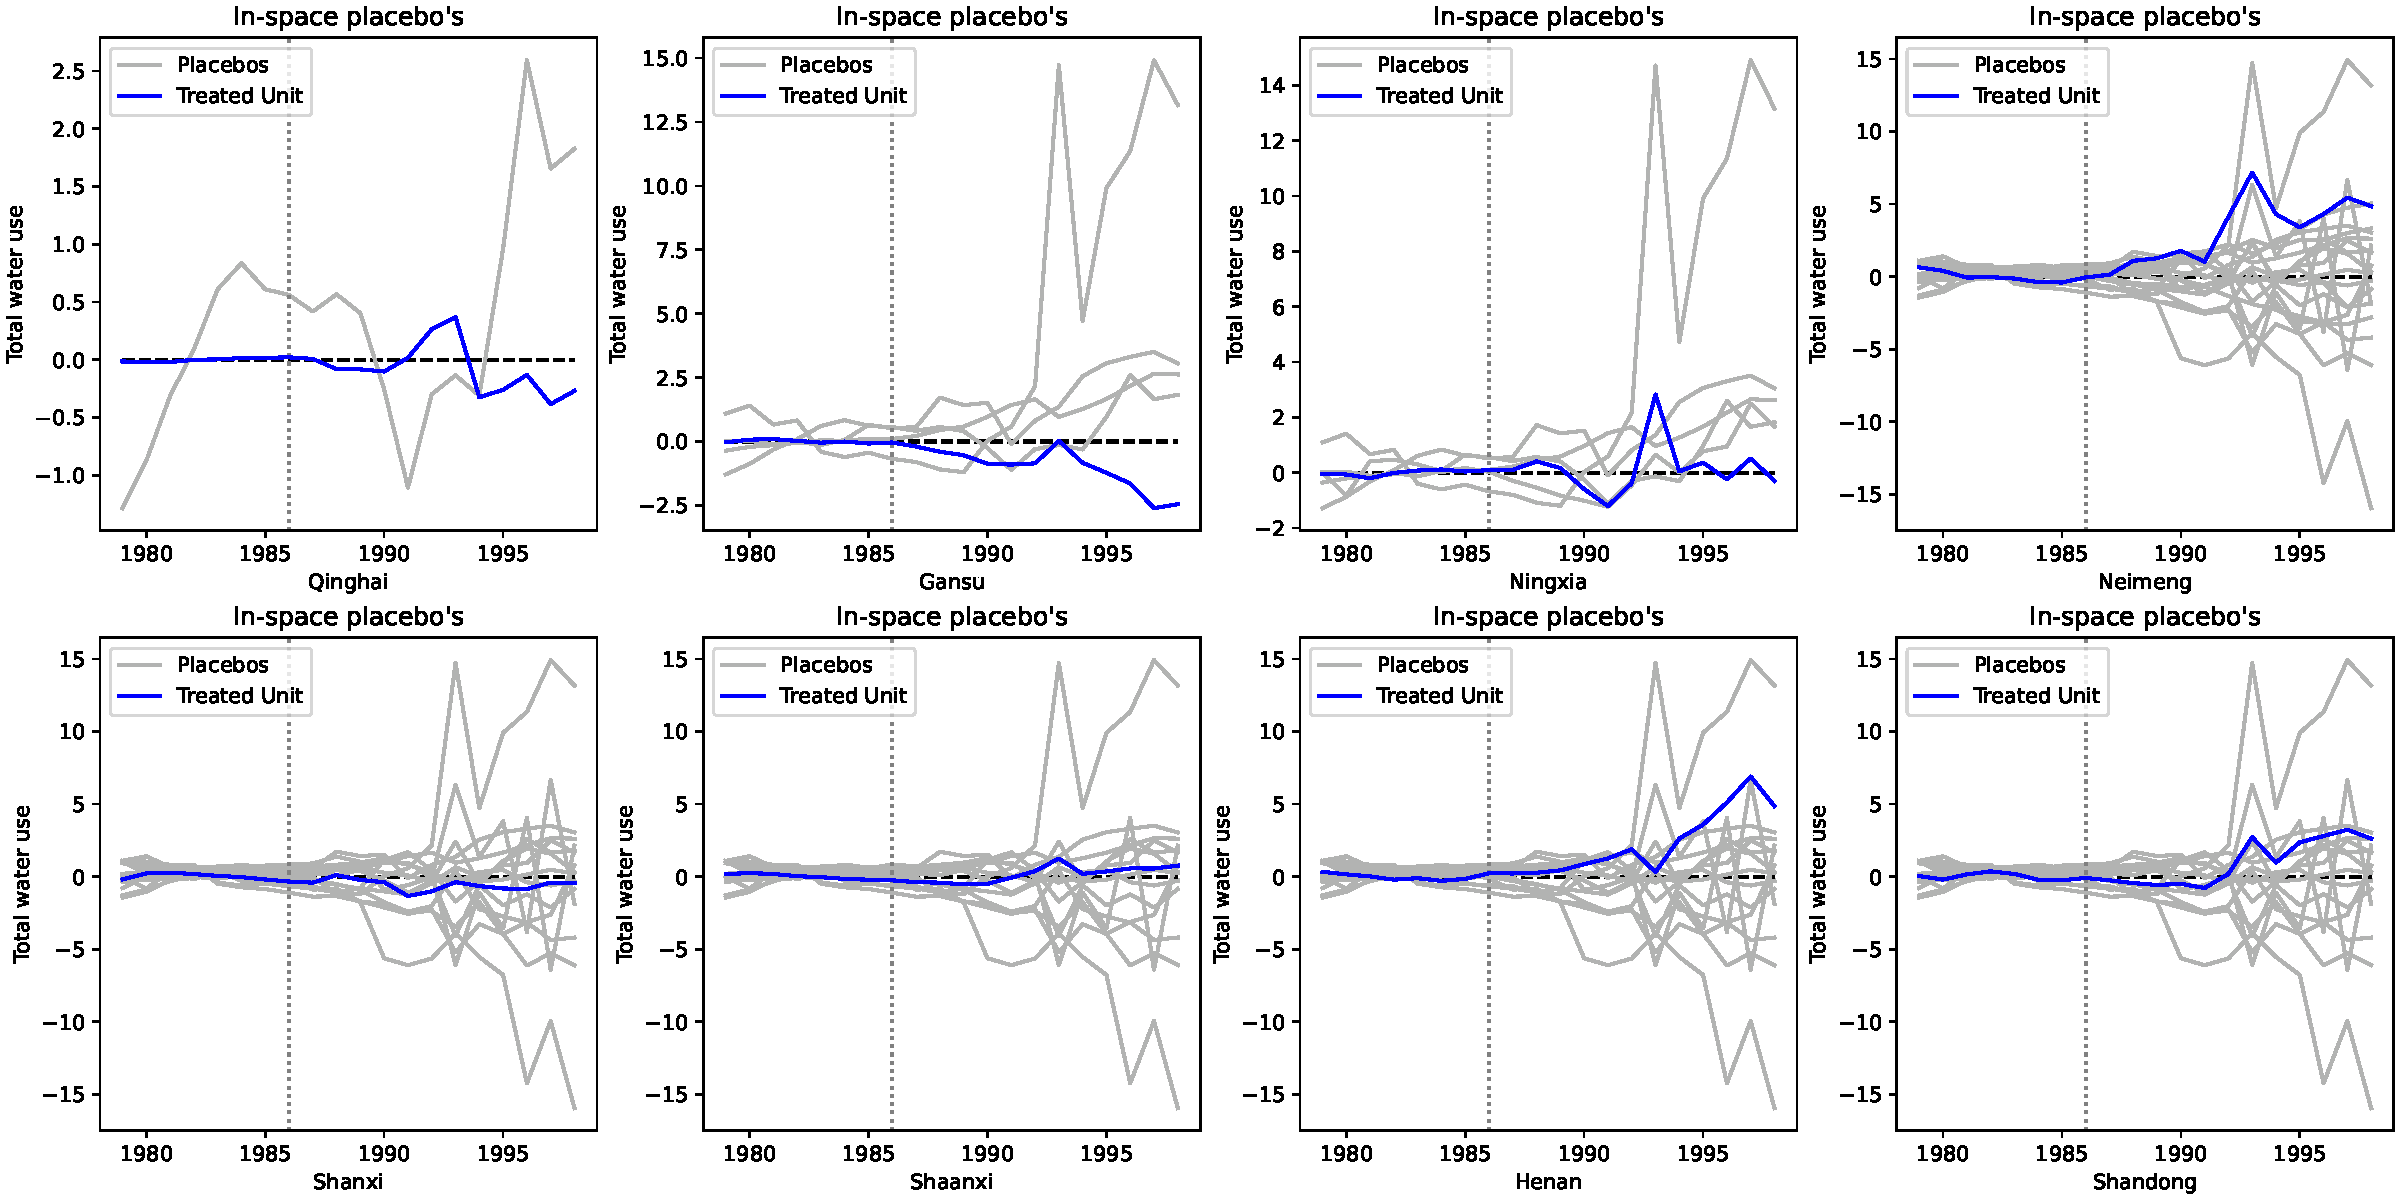
\includegraphics[width=0.9\linewidth]{img/ch5/87placebo.pdf}
    \centering
    \caption{Gaps in change in water use between provinces outside the YRB and their synthetic control, around the 87-WAS, excluding the provinces with high pre-treatment RMSPE (more than $3$ times of treated units' RMSPE).}\label{fig:87placebo}
\end{figure}

\begin{figure}
    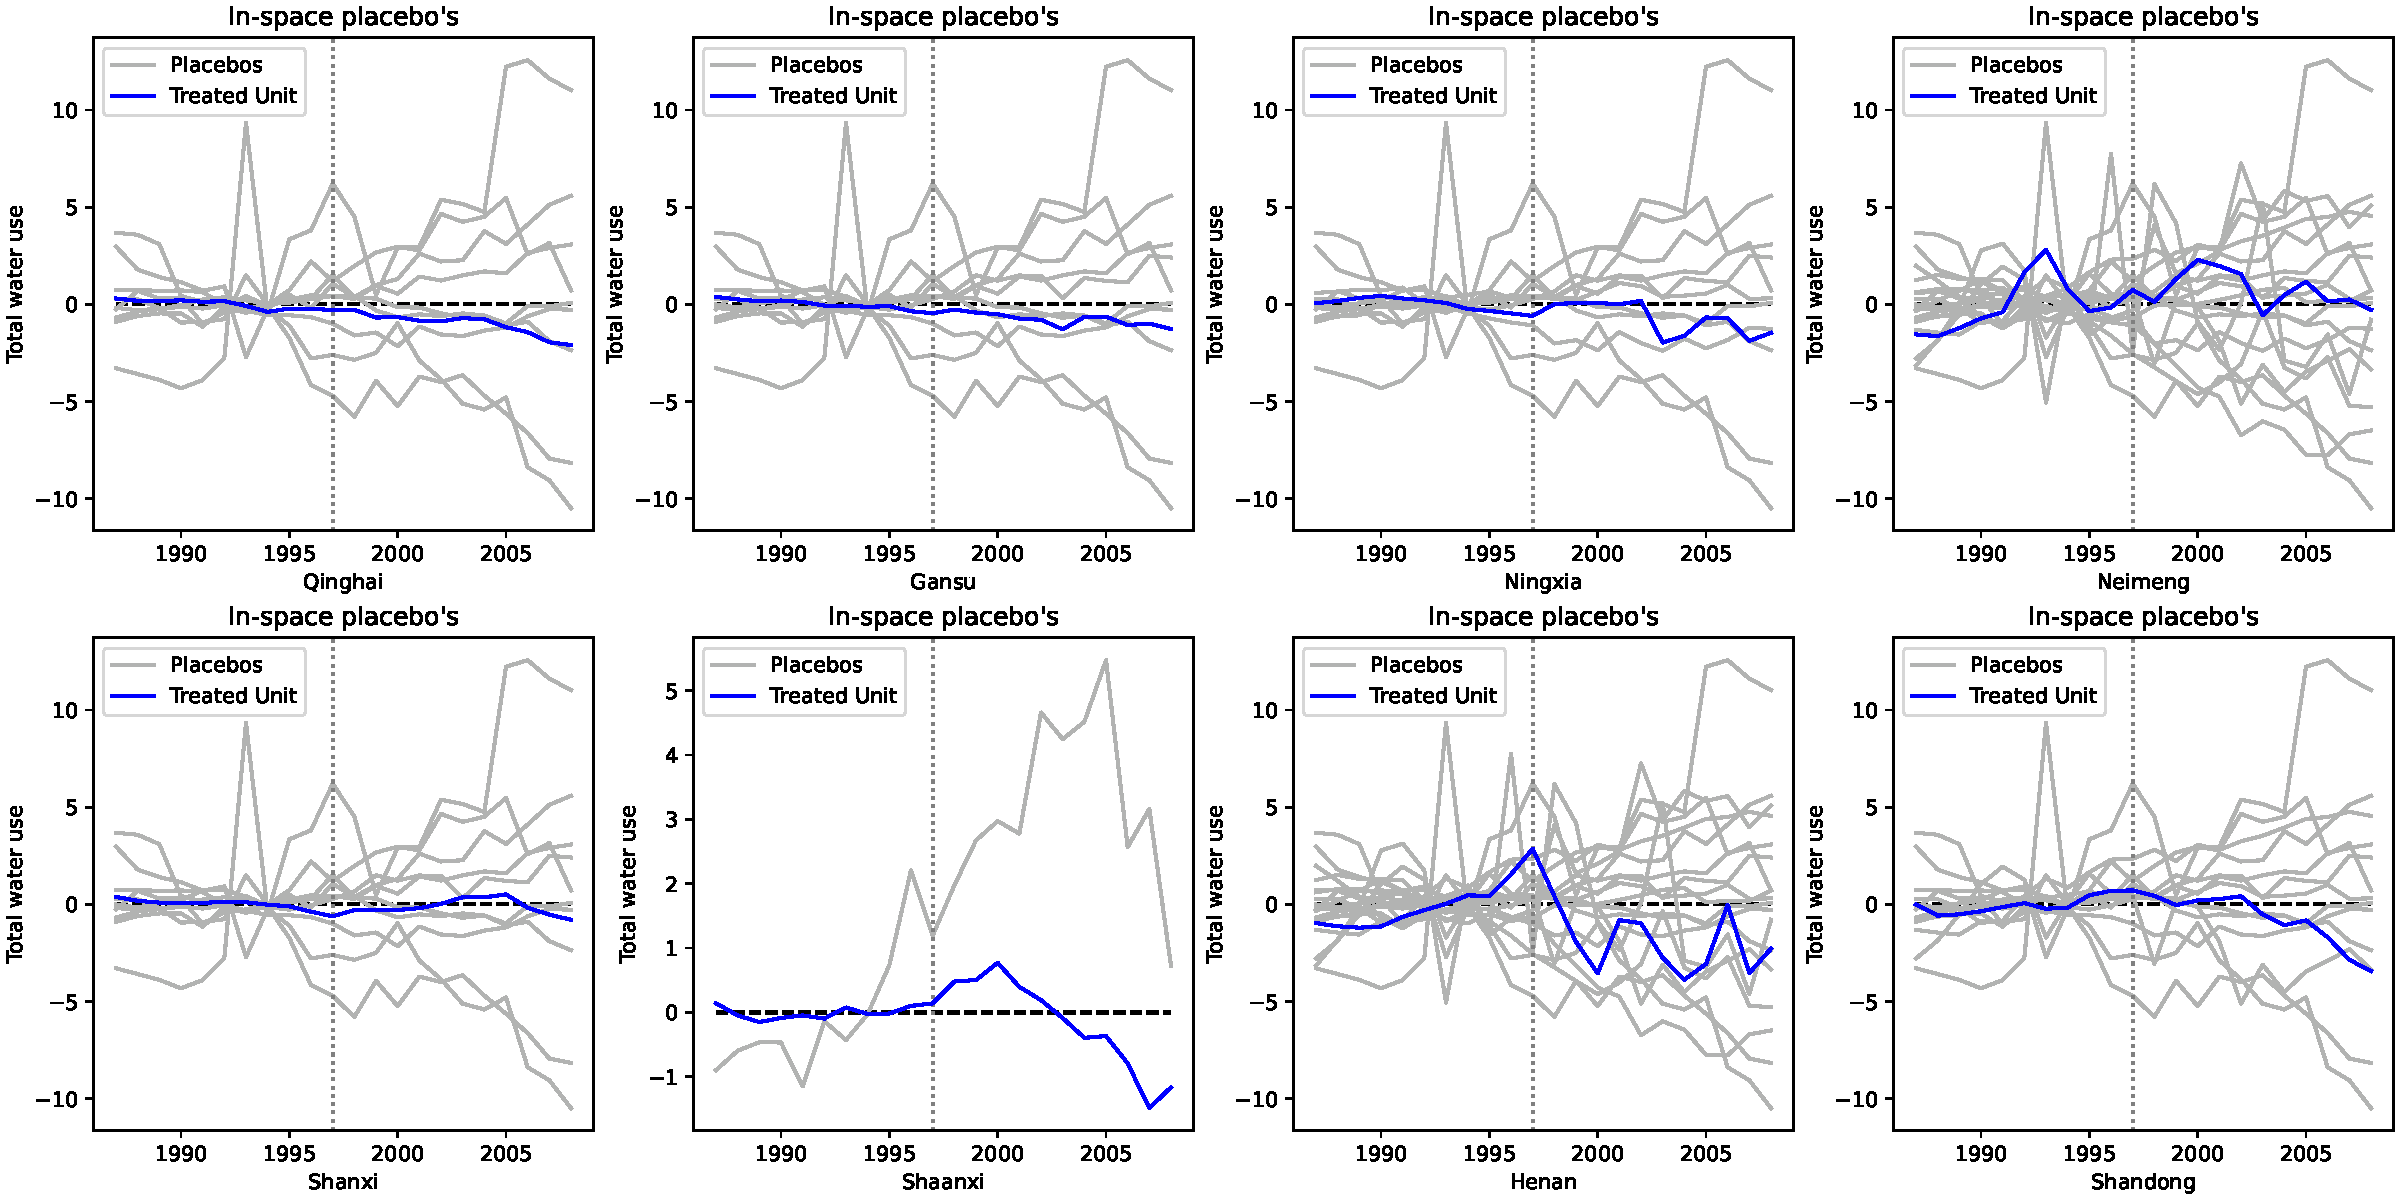
\includegraphics[width=0.9\linewidth]{img/ch5/98placebo.pdf}
    \centering
    \caption{Gaps in change in water use between provinces outside the YRB and their synthetic control, around the 98-UBR, excluding the provinces with high pre-treatment RMSPE (more than $3$ times of treated units' RMSPE)}\label{fig:98placebo}
\end{figure}
